Having decided on developing a web application, we needed to decide between a client-only or a client-server model. While a client-only would make development easier since it would not require networking, we decided to use a client-server model because the we did not want to hinder our ability to implement LPs by having to write them in JavaScript (\acrshort{js}); the most popular \acrshort{js} linear programming library on npm is jsLPSolver which at the time of writing has not been updated in over a year.

React \acrshort{js} was used for the website, as it has reusable components, state to store the visualisations, and libraries such as Material-UI to streamline development. We use TypeScript as the static type definitions and type checking will help us identify bugs.

We considered C, Java and Python to implement our server. C was favourable for its efficiency, however it lacked web server libraries. Java was considered as it supports Spring Boot, which we have previous experience using, however Spring Boot uses a controller, service, repository model. This is suited to business applications but its feature set is more extensive than we require - working within that model would slow down development. Therefore, we implemented our algorithms using Python 3 as it offered graph (NetworkX), web server (Flask) and Linear programming libraries. To supplement the lack of static typing in Python, we used type hinting.

We identified SciPy (\cite{nmeth_scipy_2020}) and Pyomo (\cite{hart_pyomo_2011}) as options for LP libraries. We implemented a prototypes for a simple linear program (\cref{fig:simple_lp}) to decide between them.

%TC:ignore
\renewcommand{\arraystretch}{0.55}
\begin{figure}[H]
    \centering
    \begin{minipage}{0.32\textwidth}
        \begin{tabularx}{\linewidth}{|rl|}
            \hline
            \multicolumn{2}{|X|}{} \tabularnewline
            maximise & $2x + 3y$\tabularnewline
            \hphantom{.......................}&\tabularnewline
            subject to & $2x + 3y \leq 9$\tabularnewline
            &\tabularnewline
            & $x,y \geq 0$\tabularnewline
            &\tabularnewline
            \hline
        \end{tabularx}%
    \end{minipage}
    \caption{Simple LP for evaluating SciPy and Pyomo}
    \label{fig:simple_lp}
\end{figure}
\renewcommand{\arraystretch}{1.0}
%TC:endignore

The two implementations are shown in \cref{fig:compare_lp}. The SciPy implementation is significantly more concise, however SciPy only supports minimisation which means in the case of maximisation, we need to inverse the signs of the variables. While the Pyomo implementation is more verbose, the constraints are more clearly defined as functions, and it has the added benefit supporting multiple solvers (SciPy is limited its own implementation of the simplex method). Therefore we use Pyomo for its clarity and its compatability with open/closed source solvers such as GLPK, Gurobi and CPLEX.

%TC:ignore
\begin{figure}[H]
    \fbox{\begin{minipage}{0.45\textwidth}
        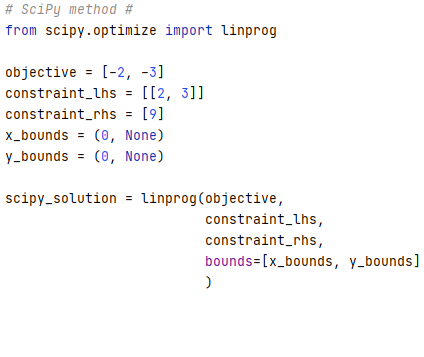
\includegraphics[height=4.8cm]{images/scipy_linprog.png}
    \end{minipage}}
    \fbox{\begin{minipage}{0.45\textwidth}
        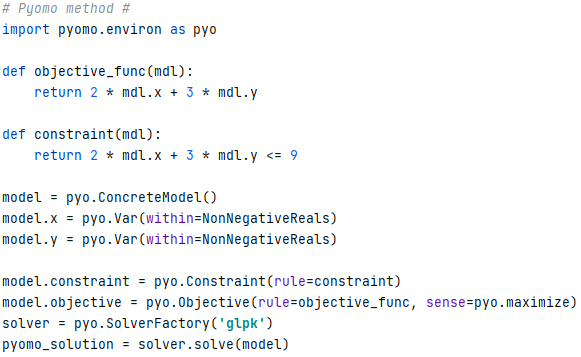
\includegraphics[height=4.8cm]{images/pyomo.png}
    \end{minipage}}
    \caption{Comparison of SciPy (left) and Pyomo (right) implementations of \cref{fig:simple_lp}}
    \label{fig:compare_lp}
\end{figure}
%TC:endignore

We also considered two libraries for visualisation: mpld3 and \acrshort{d3}.js. Mpld3 allows exporting of Matplotlib plots to \acrshort{html} . We created a basic prototype using mpld3, but we quickly found it was inflexible due to the lack of customisation for interactive legends. Furthermore for the client to render the plot in React, it would need to inject \acrshort{html} into the page which presents a potential security vulnerability. Therefore we decided to use \acrshort{d3}, a \acrshort{js} visualisation library. D3 is a more difficult library to learn since it is lower level, but it is more flexible than mpld3.